% \iffalse
\let\negmedspace\undefined
\let\negthickspace\undefined
\documentclass[beamer]{IEEEtran}
\usepackage{cite}
\usepackage{amsmath,amssymb,amsfonts,amsthm}
\usepackage{algorithmic}
\usepackage{graphicx}
\usepackage{textcomp}
\usepackage{xcolor}
\usepackage{txfonts}
\usepackage{listings}
\usepackage{enumitem}
\usepackage{mathtools}
\usepackage{gensymb}
\usepackage{comment}
\usepackage[breaklinks=true]{hyperref}
\usepackage{tkz-euclide} 
\usepackage{listings}
\usepackage{gvv}                                        
\def\inputGnumericTable{}                                 
\usepackage[latin1]{inputenc}                                
\usepackage{color}                                            
\usepackage{array}                                            
\usepackage{longtable}                                       
\usepackage{calc}                                             
\usepackage{multirow}                                         
\usepackage{hhline}                                           
\usepackage{ifthen}                                           
\usepackage{lscape}
\usepackage[export]{adjustbox}

\newtheorem{theorem}{Theorem}[section]
\newtheorem{problem}{Problem}
\newtheorem{proposition}{Proposition}[section]
\newtheorem{lemma}{Lemma}[section]
\newtheorem{corollary}[theorem]{Corollary}
\newtheorem{example}{Example}[section]
\newtheorem{definition}[problem]{Definition}
\newcommand{\BEQA}{\begin{eqnarray}}
\newcommand{\EEQA}{\end{eqnarray}}
\newcommand{\define}{\stackrel{\triangle}{=}}
\theoremstyle{remark}
\newtheorem{rem}{Remark}
\begin{document}
\parindent 0px
\bibliographystyle{IEEEtran}

\title{Assignment\\[1ex]11.9.1 - 9}
\author{EE23BTECH11220 - R.V.S.S Varun$^{}$% <-this % stops a space
}
\maketitle
\newpage
\bigskip

\renewcommand{\thefigure}{\theenumi}
\renewcommand{\thetable}{\theenumi}
\section*{Question}
Find $a_{9}$ in the sequence $a_{n}=\brak{-1}^{n-1}n^{3}$ 
\section*{Solution}
 
\begin{table}[h]
    \centering
   \begin{tabular}{|c|c|c|}
        \hline
	Symbol &Value&Description \\
        \hline
	 x\brak{0}&12&First term of the series \\
         \hline
	 x\brak{n}&4\brak{n+1}\brak{n+2}u\brak{n}&$\brak{n+1}^{th}$ term of the series  \\
         \hline
         
    \end{tabular}

    
    \caption{Table of parameters}
    \label{tab:11.9.1.9.1}
\end{table}


To obtain $9^{th}$ term of the sequence put $n$=8 in x\brak{n}
\begin{align}
x\brak{8}=729
\end{align}
From up-scaling property,
\begin{align}
x\brak{n}\xleftrightarrow{\mathcal{Z}} X\brak{z} \\
x\brak{kn}\xleftrightarrow{\mathcal{Z}} X\brak{z^k}
\end{align}
From table,
\begin{align}
	x\brak{2n}=\brak{2n+1}^{3}u\brak{2n}
\end{align}
Using  $Z$ transform,
\begin{align}
	x\brak{n}\xleftrightarrow{\mathcal{Z}}X\brak{z}\\
	x\brak{2n}\xleftrightarrow{\mathcal{Z}}X\brak{z^2}
\end{align}


\begin{align}
	u\brak{2n}\xleftrightarrow{\mathcal{Z}}\frac{1}{\brak{1-z^{-2}}},\abs{z}>1 
\end{align}

\begin{align}
	{2n} \hspace{5pt} u\brak{2n} \xleftrightarrow{\mathcal{Z}} \frac{z^{-2}}{\brak{1-z^{-2}}^2},\abs{z} >1 \\
    \brak{2n}^2  u\brak{2n} \xleftrightarrow{\mathcal{Z}} \frac{z^{-2}\brak{z^{-2}+1}}{\brak{1-z^{-2}}^3},\abs{z} > 1 \\
	\brak{2n}^3 u\brak{2n} \xleftrightarrow{\mathcal{Z}}  \frac{z^{-2}\brak{1+4z^{-2}+z^{-4}}}{\brak{1-z^{-2}}^4},\abs{z} >1
\end{align}
\begin{align}
	X\brak{z^2} &=\sum_{n=-\infty}^{n=\infty}\brak{2n+1}^{3}u\brak{2n}z^{-2n}
\end{align}
\begin{align}
	&=\sum_{n=-\infty}^{n=\infty}\brak{\brak{2n}^3+3\brak{2n}^2+3\brak{2n}+1}u\brak{2n}z^{-2n}\hspace{10pt}
\{z:|z|>1\}
\end{align} 
\begin{align}
	&=\frac{4z^6+z^4-3z^2}{\brak{z^2-1}^4}, \abs{z}>1 
\end{align}
Replace $z^2$ by $z$ in \brak{14}
\begin{align}
	X\brak{z}=\frac{4z^3+z^2-3z}{\brak{z-1}^4} , \abs{z}>1
\end{align}

\begin{figure}[h]
    \centering
    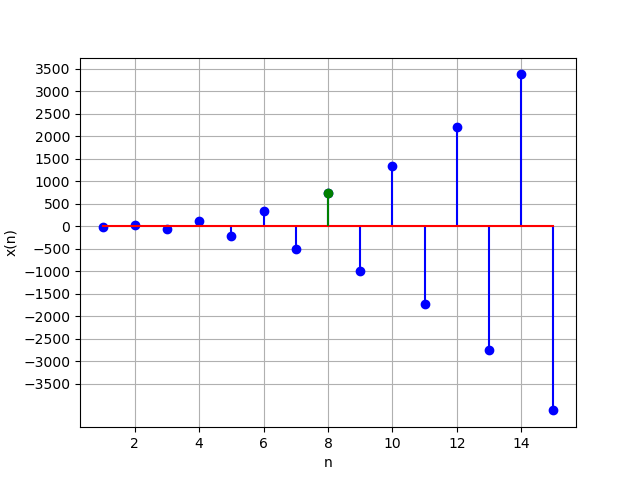
\includegraphics[width=1 \columnwidth]{figs/graph.png} 
    \label{fig:11.9.1.9.1}
\end{figure}
\begin{center}
Graph of x\brak{n}
   \end{center}
\end{document}
